\documentclass[12pt,a4paper]{article}

\usepackage[margin=1in]{geometry}
\usepackage{graphicx}
\usepackage{verbatim}
\usepackage{iftex}
\usepackage{float}
\usepackage[hidelinks]{hyperref}
\urlstyle{same}
\sloppy

\ifPDFTeX
  \usepackage{helvet}
  \renewcommand{\familydefault}{\sfdefault}
\else
  \usepackage{fontspec}
  \setmainfont{Arial}
  \setsansfont{Arial}
  \setmonofont{Menlo}
\fi

\makeatletter
\renewcommand\section{\@startsection{section}{1}{\z@}%
  {-3.5ex \@plus -1ex \@minus -.2ex}%
  {2.3ex \@plus .2ex}%
  {\normalfont\bfseries\fontsize{14}{16}\selectfont}}
\renewcommand\subsection{\@startsection{subsection}{2}{\z@}%
  {-3.25ex \@plus -1ex \@minus -.2ex}%
  {1.5ex \@plus .2ex}%
  {\normalfont\bfseries\fontsize{12}{14}\selectfont}}
\makeatother

\title{CPT304 Coursework 1 Report\\Taskify Research-Led Software Enhancement}
\author{Group XX}
\date{May 2026}

\begin{document}
\maketitle

\section{App Selection}
Taskify was chosen because it is a task-management app with a simple user journey: a visitor signs up or logs in, then manages tasks on the dashboard. That made it practical to audit the project from the page templates through to the Express routes and tests. The app was also not already polished to the coursework baseline. It had issues in accessibility, backend form handling, persistence, test coverage, and compliance pages. Those gaps made it a good project for small, traceable fixes rather than a broad rewrite.

\section{Authentication Form Fields Relied on Placeholder Text}

\subsection{Detection}
The issue was first found while checking \texttt{views/signup.ejs}. The sign-up and login inputs had placeholder text, but the user-entered fields did not have their own visible labels or matching \texttt{id}/\texttt{for} pairs. This was easy to miss because the page looked acceptable before typing. The problem appeared once text was entered: the placeholder disappeared, leaving the filled username field without a visible field name. The browser evidence in Figure~\ref{fig:auth-form-labels} shows that exact before and after state.

\subsection{Literature}
WCAG 2.2 Success Criterion 3.3.2 requires labels or instructions when content needs user input \cite{wcag-332}. W3C Technique H44 gives the implementation detail used here: explicit \texttt{label} elements can be connected to controls through matching \texttt{for} and \texttt{id} values, and visible labels also help users understand the field before and after typing \cite{w3c-h44}. This made the fix semantic rather than only visual.

\subsection{Implementation}
The original field relied on the placeholder to describe the input:

\noindent\textbf{Before fix: placeholder-only email field.}
{\footnotesize
\begin{verbatim}
<input type="email" name="SignUpEmail"
  placeholder="Email" required="true" />
\end{verbatim}
}

The updated page keeps the hint text, but adds a real label and a stable association:

\noindent\textbf{After fix: visible label connected to the input.}
{\footnotesize
\begin{verbatim}
<label class="field-label" for="signup-email">Email</label>
<input id="signup-email" type="email" name="SignUpEmail"
  autocomplete="email" placeholder="Email" required />
\end{verbatim}
}

The same pattern was applied to the username, password, login email, and login password fields. The CSS was also split so the large panel switch labels use \texttt{.toggle-label}, while normal input labels use \texttt{.field-label}. That avoided turning every form label into a page heading. The final result keeps the field name visible after typing and gives assistive technology a clear label-to-control relationship.

\begin{figure}[H]
  \centering
  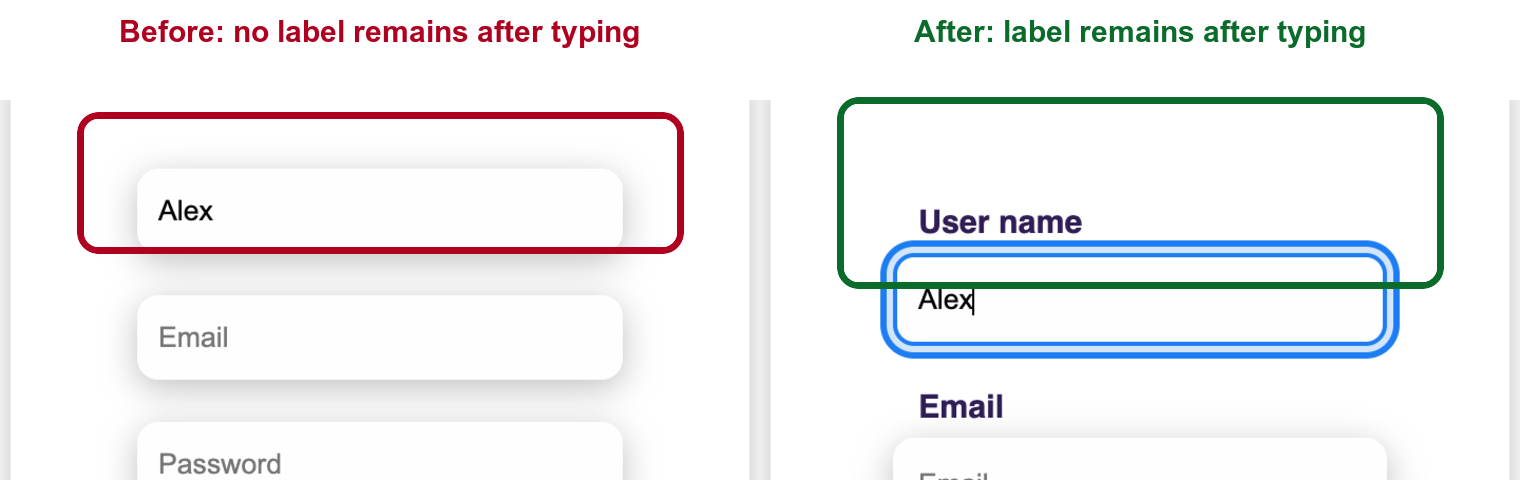
\includegraphics[width=0.92\linewidth]{figures/auth-form-labels-before-after.png}
  \caption{Authentication form label evidence. Before the fix, the username placeholder disappears after typing and no field label remains. After the fix, the visible ``User name'' label stays above the filled input.}
  \label{fig:auth-form-labels}
\end{figure}

\section{Authentication Forms Submitted to Missing Backend Routes}

\subsection{Detection}
The next issue came from following the same forms through to the backend. In \texttt{views/signup.ejs}, the sign-up form submitted \texttt{POST /signup} and the login form submitted \texttt{POST /login}. In the earlier \texttt{src/app.js}, Express only defined \texttt{GET /}, \texttt{GET /signup}, and \texttt{GET /dashboard}. A direct curl check confirmed the bug: a valid \texttt{POST /signup} returned \texttt{HTTP/1.1 404 Not Found}. In practice, a user could fill the form correctly and still be sent to a missing route.

\subsection{Literature}
Express routing is matched by both HTTP method and path, so \texttt{GET /signup} does not handle \texttt{POST /signup} \cite{express-routing}. OWASP's Input Validation Cheat Sheet was used because direct POST requests can bypass browser validation, so required fields and email format still need server-side checks \cite{owasp-input-validation}. RFC 9110 was used for the success path: \texttt{303 See Other} redirects the user agent to a different resource identified by the \texttt{Location} header, which fits a Post/Redirect/Get flow to \texttt{/dashboard} \cite{rfc9110}.

\subsection{Implementation}
The earlier backend rendered the sign-up page but did not process its submission:

\noindent\textbf{Before fix: sign-up page existed, but no POST handler existed.}
{\footnotesize
\begin{verbatim}
app.get("/signup", (req, res) => {
    res.status(200).render("signup.ejs");
});
\end{verbatim}
}

The fix added method-specific POST handlers for the existing form actions:

\noindent\textbf{After fix: server-side validation and Post/Redirect/Get.}
{\footnotesize
\begin{verbatim}
app.post("/signup", (req, res) => {
    const missingFields = collectMissingFields(req.body, [
        "SignUpUsername", "SignUpEmail", "SignUpPassword",
    ]);

    if (missingFields.length > 0 || !isValidEmail(req.body.SignUpEmail)) {
        return res.status(400).json({
            success: false,
            errors: {
                missingFields,
                email: isValidEmail(req.body.SignUpEmail) ? undefined
                    : "Enter a valid email address.",
            },
        });
    }

    return res.redirect(303, "/dashboard");
});
\end{verbatim}
}

The same approach was added for \texttt{POST /login}. The app now rejects invalid email input with \texttt{400 Bad Request} and redirects valid submissions with \texttt{303 See Other}. To make this testable, \texttt{src/app.js} exports the Express app and only starts \texttt{listen()} when run directly, so \texttt{node --test} can run the route checks on a temporary port.

\begin{figure}[H]
  \centering
  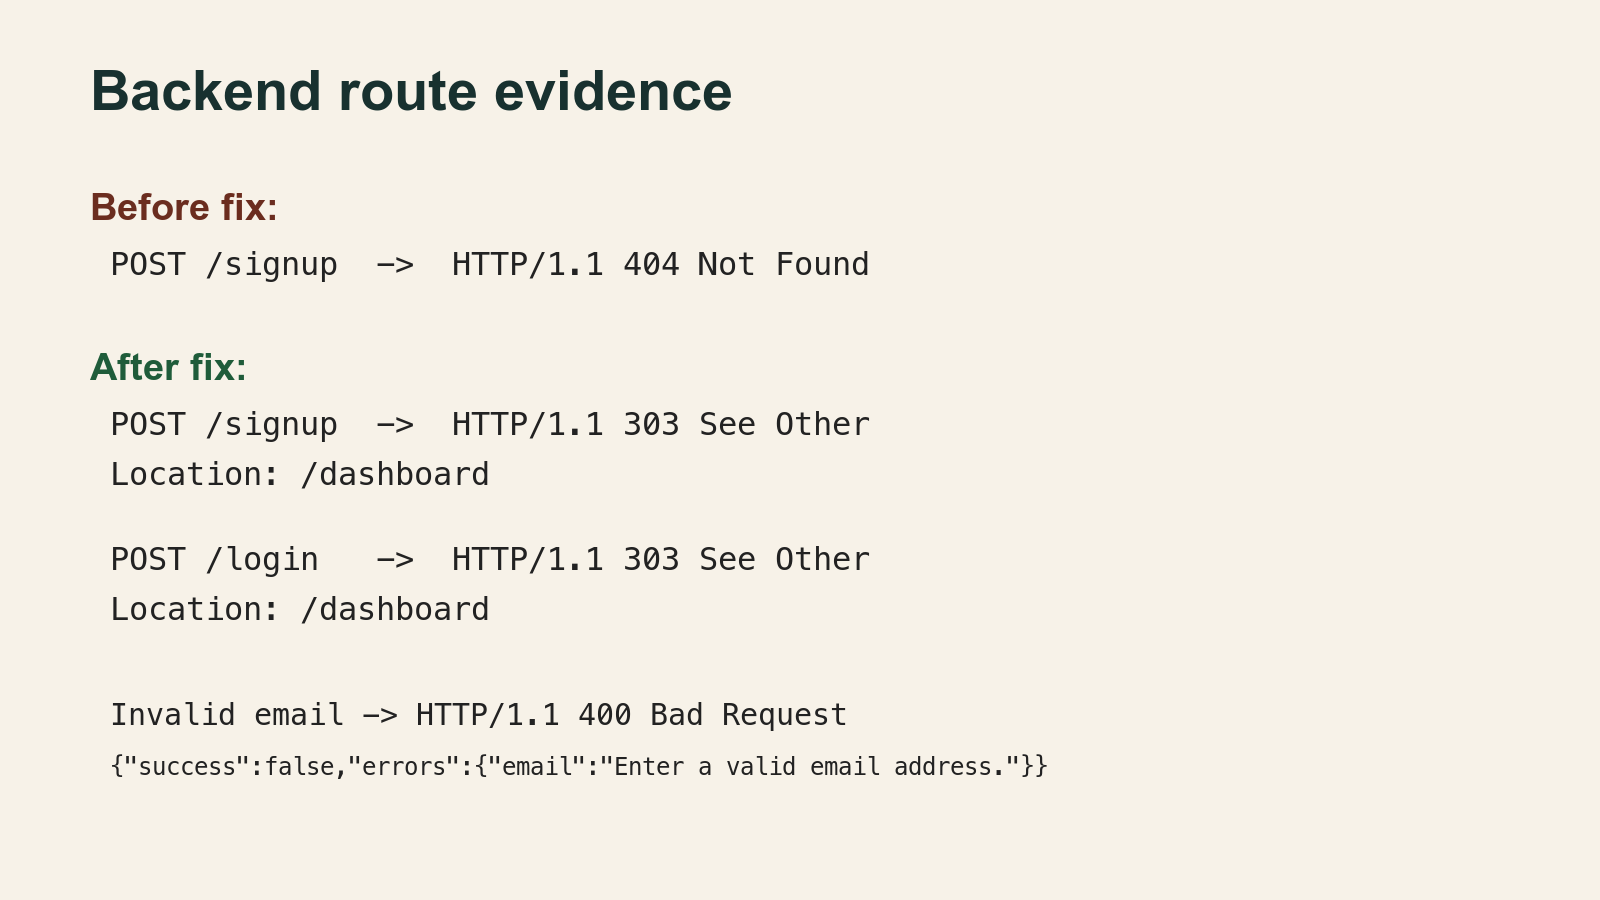
\includegraphics[width=0.92\linewidth]{figures/auth-http-evidence.png}
  \caption{Backend route evidence. Before the fix, a valid \texttt{POST /signup} returned 404. After the fix, valid sign-up and login submissions return \texttt{303 See Other} to \texttt{/dashboard}, while invalid email input is rejected with \texttt{400 Bad Request}.}
  \label{fig:auth-http-evidence}
\end{figure}

\section{Dashboard Tasks Were Lost After Refresh}

\subsection{Detection}
The third issue appeared during a refresh check on the dashboard task board. A new task could be created and shown on the board, but after refreshing the page the board went back to the three sample tasks. The saved item, \texttt{Persistence evidence task}, was gone. The cause was in \texttt{static/js/dashboard.js}: the initial task state was rebuilt from \texttt{seedTasks} every time the script loaded, and the updated task array was not written anywhere durable. Figure~\ref{fig:persistence-refresh} shows the full check: the task first exists after saving, then disappears after refresh in the old version, and finally remains after refresh in the fixed version.

\subsection{Literature}
MDN describes the Web Storage API as a browser feature for storing key-value data on the client, with \texttt{localStorage} persisting beyond a single page session \cite{mdn-web-storage}. The W3C Web Storage specification defines \texttt{getItem} and \texttt{setItem} as origin-scoped storage operations, so it was a reasonable fit for a small dashboard task list that did not yet have a database-backed task model \cite{w3c-web-storage}. The loader still needed a safe fallback, because browser storage can be empty, cleared, or contain invalid JSON. In those cases, the dashboard should return to the sample tasks instead of failing to render.

\subsection{Implementation}
The earlier dashboard always rebuilt state from the same seed data:

\noindent\textbf{Before fix: dashboard state was recreated on every load.}
{\footnotesize
\begin{verbatim}
let state = {
  tasks: seedTasks.map((task) => ({ ...task })),
};

function deleteTask(taskId) {
  state.tasks = state.tasks.filter((task) => task.id !== taskId);
  renderBoard();
  showMessage("Task deleted successfully.");
}
\end{verbatim}
}

The fix moved persistence into a small module and loaded the dashboard from \texttt{localStorage} when valid saved data exists:

\noindent\textbf{After fix: state is loaded safely and saved after changes.}
{\footnotesize
\begin{verbatim}
import { persistTasks, safeLoadTasks } from "./modules/task-store.mjs";

let state = {
  tasks: safeLoadTasks(window.localStorage,
    seedTasks.map((task) => ({ ...task }))).tasks,
};

function persistState() {
  persistTasks(window.localStorage, state.tasks);
}

function deleteTask(taskId) {
  state.tasks = state.tasks.filter((task) => task.id !== taskId);
  persistState();
  renderBoard();
}
\end{verbatim}
}

The new \texttt{task-store.mjs} file keeps the storage key in one place and wraps \texttt{JSON.parse} in a \texttt{try}/\texttt{catch}. If saved data is missing, invalid JSON, or not an array, \texttt{safeLoadTasks} returns the fallback seed tasks instead of throwing an error. The dashboard now calls \texttt{persistState()} after save, delete, and move actions. The page script was also changed to \texttt{type="module"} so the dashboard can import the storage helper cleanly.

\begin{figure}[H]
  \centering
  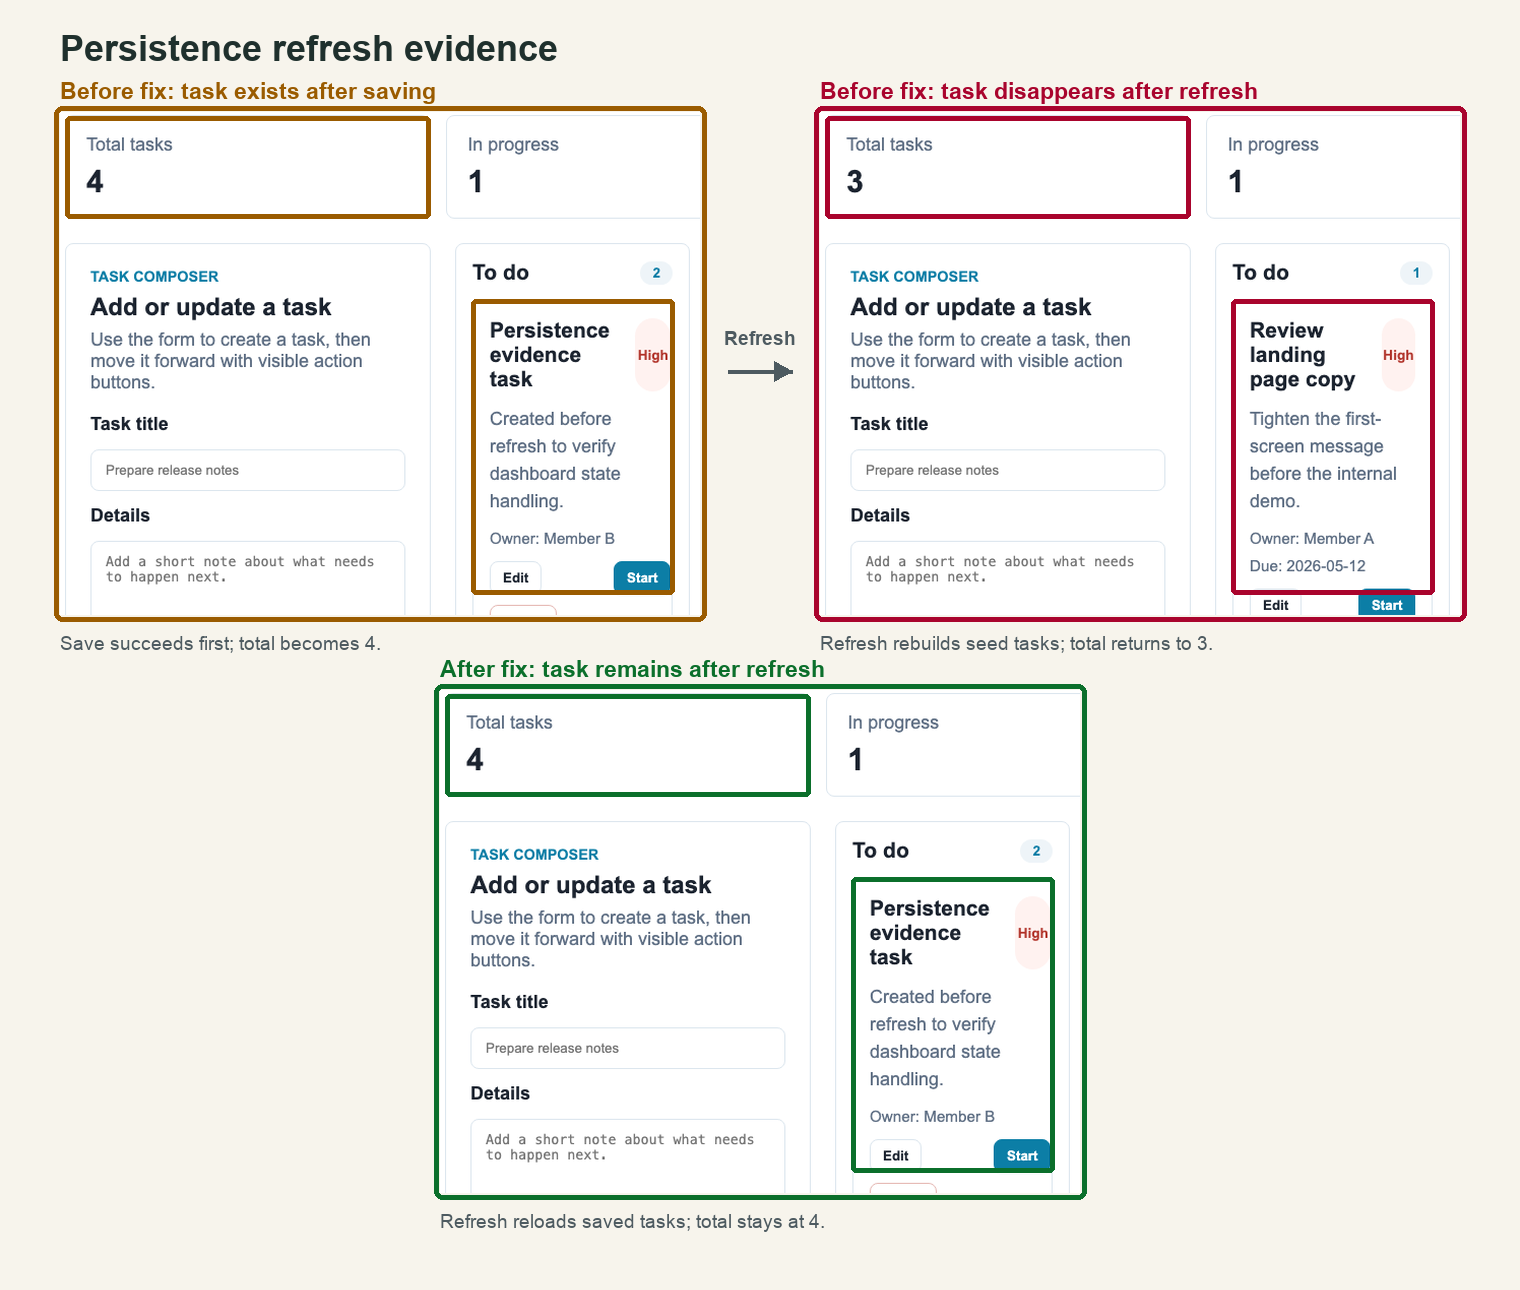
\includegraphics[width=0.96\linewidth]{figures/persistence-refresh-before-after.png}
  \caption{Persistence refresh evidence. The first pre-fix panel shows that the task was created successfully before refresh. The second pre-fix panel shows the defect: refreshing the dashboard rebuilds the board from seed tasks, so the total returns to three and the saved task is missing. After the fix, the same refresh keeps the saved task because the board reloads the \texttt{localStorage} task list.}
  \label{fig:persistence-refresh}
\end{figure}

\section{Deficiency 4 Placeholder}
\textbf{TODO:} Insert the fourth completed deficiency. Include detection method, literature source, implementation rationale, and real before-vs-after code.

\section{Baseline Standards Evidence}
\textbf{TODO:} Add concise evidence and screenshots for the required baseline standards: 7-day Vercel/Render uptime, Codecov/Istanbul coverage of at least 80\%, Lighthouse Accessibility score of at least 90, a two-language i18n toggle, a cookie banner, and a privacy policy page. Each screenshot must have a figure number and descriptive caption.

\section{Individual Contribution Forms}
The completed contribution workbook is included as a separate submission artifact: \texttt{individual-contribution.xlsx}. This file is excluded from the report word count and is the place where individual contribution evidence and pull-request links are recorded.

\section{References}
\renewcommand{\refname}{}
\vspace{-2em}
\begin{thebibliography}{9}
\bibitem{wcag-332} W3C Web Accessibility Initiative, ``Understanding Success Criterion 3.3.2: Labels or Instructions.'' [Online]. Available: \url{https://www.w3.org/WAI/WCAG22/Understanding/labels-or-instructions.html}. Accessed: May 8, 2026.
\bibitem{w3c-h44} W3C Web Accessibility Initiative, ``H44: Using label elements to associate text labels with form controls.'' [Online]. Available: \url{https://www.w3.org/WAI/WCAG22/Techniques/html/H44}. Accessed: May 8, 2026.
\bibitem{express-routing} Express, ``Routing.'' [Online]. Available: \url{https://expressjs.com/en/guide/routing.html}. Accessed: May 8, 2026.
\bibitem{owasp-input-validation} OWASP Cheat Sheet Series, ``Input Validation Cheat Sheet.'' [Online]. Available: \url{https://cheatsheetseries.owasp.org/cheatsheets/Input_Validation_Cheat_Sheet.html}. Accessed: May 8, 2026.
\bibitem{rfc9110} R. Fielding, M. Nottingham, and J. Reschke, ``HTTP Semantics,'' RFC 9110, Jun. 2022. [Online]. Available: \url{https://www.rfc-editor.org/rfc/rfc9110}. Accessed: May 8, 2026.
\bibitem{mdn-web-storage} MDN Web Docs, ``Web Storage API.'' [Online]. Available: \url{https://developer.mozilla.org/en-US/docs/Web/API/Web_Storage_API}. Accessed: May 8, 2026.
\bibitem{w3c-web-storage} W3C, ``Web Storage (Second Edition).'' [Online]. Available: \url{https://www.w3.org/TR/webstorage/}. Accessed: May 8, 2026.
\end{thebibliography}

\end{document}
